\chapter{Gekozen concept}
\label{cha:gekozenConcept}

\textit{In dit hoofdstuk worden verbeterrichtingen aangewezen in het huidige ontwerp, worden de verbeteringen toegepast en wordt dit verbeterde ontwerp  geanalyseerd. Eerst worden verbeterrichtingen aangewezen vanuit het programma van eisen (\cref{se:PVE}). Dan worden deze richtingen aangevuld door het maken van een proefmodel en het uitvoeren van een veiligheidsanalyse (\ref{se:Veiligheidsanalyse}) en een faalanalyse (\cref{se:Faalanalyse}). Het verbeterde concept wordt dan toegelicht. Ten slotte wordt het verbeterde concept geanalyseerd op gewicht en bewegingsvrijheid (\cref{se:Verbeterd_concept}).}


\section{Verbeterrichtingen}
 Nadat er een keuze is gemaakt tussen de verschillende kansrijke concepten is (\cref{cha:Concept_keuze}), werd er gekeken naar hoe dit concept nog verbetert kon worden op verscheidene manieren. De pootjes die het oorspronkelijke concept bevatte, zijn veranderd voor schaarliften. Deze schaarliften staan dwars op de basis en kunnen worden bestuurd door middel van een steppermotor. 
 
 Er is gekozen voor een steppermotor, aangezien de verticale verplaatsing van de verschillende schaarliften hiermee nauwkeurig kan worden bepaald en het pakketje zo horizontaal mogelijk kan worden gehouden. De schaarliften zelf hebben als voordeel dat de hoogte van het concept hiermee kan worden veranderd, wat met de pootjes niet mogelijk was. Hierdoor is er geen extra schaarlift bovenop het concept nodig om het pakketje te kunnen ontvangen en afleveren en is het concept op deze manier een stuk simpeler geworden. Ook is het realiseren van de verticale verplaatsing met schaarliften makkelijker en was voor het omhoog- en omlaaghalen van de pootjes een redelijk ingewikkeld systeem nodig. 
 
 Voor het stuurmechanisme maakt de driepoter gebruik van het Ackermann-principe dat ook in het concept van de inklapper wordt gebruikt, zie \cref{fig:vierpoter_stuursysteem}. Het mechanisme van de wielaandrijving wordt overgenomen van de vierpoter, dit wordt afgebeeld in \cref{fig:vierpoter_aandrijving}. 
 
 \section{Veiligheidssanalyse en faalanalyse concept}
Naast een analyse van de werking van het concept, moet er uiteraard ook naar de veiligheid en faalmechanismen worden gekeken. In \cref{se:Veiligheidsanalyse} is er een analyse gedaan rondom de veiligheid van het concept. In \cref{se:Faalanalyse} is er een analyse gedaan rondom de verschillende faalemechanismen, waarbij er is gekeken naar waarschijnlijkheid van optreden en ernst van falen.

 \subsection{Veiligheidsanalyse}
 \label{se:Veiligheidsanalyse}
 Op gebied van veiligheid is er vooral aandachtig gekeken naar uitstekende en scherpe delen. 

Ten eerste werd er gekeken naar gevaren tijdens het fabriceren. In gesloten machines die door een computer wordt bestuurd, zoals een dxf snijmachine, zijn weinig gevaren. Er is weinig tot geen interactie met het materiaal zelf door de persoon. Bij bijvoorbeeld de draai- of freesmachine moet er uiteraard worden gekeken naar de bijbehorende veiligheidsvoorschriften, zoals een veiligheidsbril en een correcte jas. Er zullen ook dingen gelast moeten worden, met de bijbehorende lashelm en bedekkende kleding zou dit tot geen enkel probleem moeten lijden, er wordt extra gelet op verbrandingsgevaar (van ogen en huid). Met andere onderdelen wordt rekening gehouden dat deze niet dusdanig klein zijn dat het gevaarlijk wordt met groot gereedschap te bewerken. Na elke snij bewerking, of bij het aantreffen van een scherpe rand, wordt deze onmiddellijk geschuurd tot het de huid niet meer kan snijden.

De meeste onderdelen kunnen veilig gemonteerd worden, er zijn voornamelijk in elkaar schuivende onderdelen of in elkaar draaiende onderdelen, hier wordt geen gevaar in gezien.

Ten derde is er grondig gekeken naar de veiligheid tijdens het gebruik. Er zijn geen uitstekende onderdelen, en scherpe randen zijn keurig geschuurd of anders omgebogen. Een punt om tijdens werking op te letten zijn de schaarliften. Bij het inklappen moeten handen/voeten van de schaarlift vandaan blijven. Als het metaal naar elkaar toe beweegt ziet de steppermotor geen verschil als er er iets tussen is en kan dit verwondingen opleveren.

 
\subsection{Faalanalyse}
\label{se:Faalanalyse}
Er zijn verschillende manieren waarop het concept kan falen, maar met niet veel moeite kan met deze scenario's rekening gehouden worden en kan het risico op falen laag zijn.

Bij het driepotige concept bevindt het pakketje zich op een beweegbaar dek, hier is de kans op falen het grootst. Het dek wordt handmatig bestuurd door te trekken aan een touwtje. Dit betekend dat ten eerste het dek kan loskomen waardoor het pakketje niet meer wordt vervoerd door het pakket hondje.

Daarnaast kan er door het fout verplaatsen van het pakket hondje het zwaartepunt zich naar de verkeerde kant bewegen, dit betekent dat het gehele pakket hondje omvalt bij het nemen van een obstakel. Bij het uitoefenen van de werking van het pakket hondje kan het risico op een foute verplaatsing sterk worden verkleind. Het is dus van groot belang dat alleen personen die het concept voldoende begrijpen deze besturen.

Een ander gevaarlijk punt op falen is het bezwijken van de schaarliften onder gewicht. Dit zou betekenen het pakketje überhaupt niet kan worden overgebracht en geen obstakel zou kunnen nemen. Hierom zou hier de grootste veiligheidsmarge op moeten worden genomen. Ook al zou bij een normale veiligheidsmarge het risico niet groot zijn zou dit het gehele project kunnen ondermijnen. Er moet dus een berekening gemaakt worden om te zien of het huidige ontwerp nog aangepast moet worden voor het eindontwerp geproduceerd kan worden.
\begin{figure}[H]
    \centering
    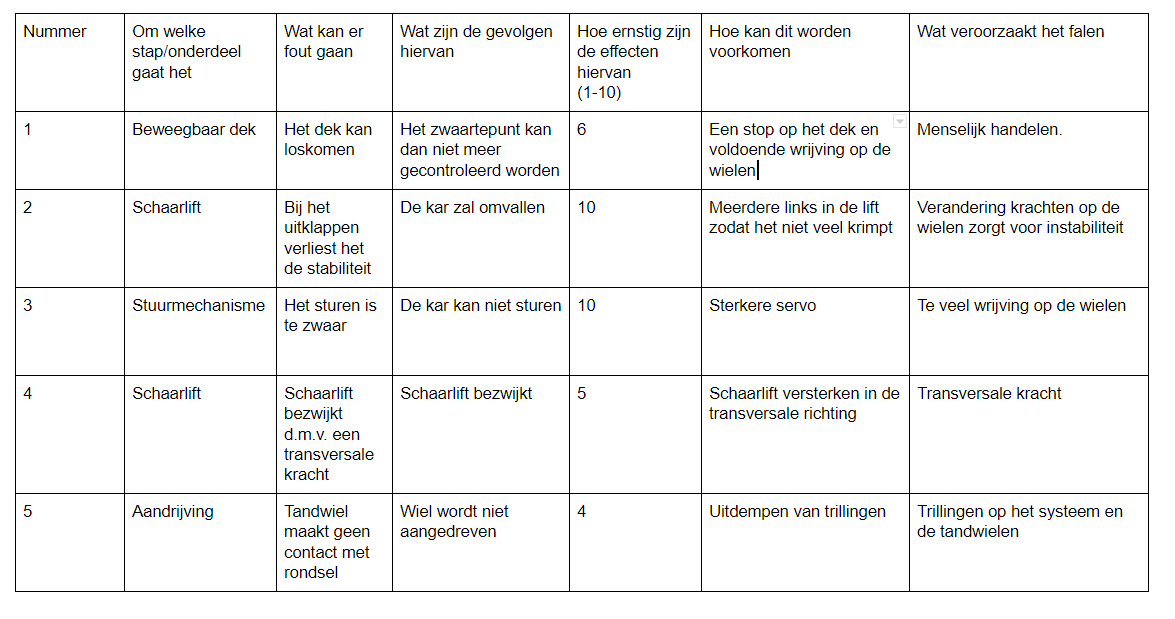
\includegraphics[width = 150mm]{04_gekozenconcept/Tabel_faal.PNG}
    \caption{Faalanalyse van de kar}
    \label{fig:tabel_faal}
\end{figure}

\section{Verbeterd concept}
\label{se:Verbeterd_concept} 
Bij dit ontwerp moet er rekening worden gehouden met de verplaatsing van het zwaartepunt, dit gebeurt door het implementeren van een schuifsysteem uit het ontwerp van de vierpoter. Dit schuifsysteem heeft een dubbele functie, namelijk: verschuiven van het zwaartepunt en bewegen van het pakketje, zie \cref{fig:driepoter_SW} voor verheldering op het mechanisme. 

Door het model in solidworks te maken is de massa van het ontwerp bekend. Volgens solidworks is dit ongeveer 8kg. Dit is minder dan het pakket, wat betekend dat het zwaartepunt van het ontwerp makkelijk aangepast kan worden door het bewegen van het pakket.

Ook kan de bewegingsvrijheid van het model ingeschat worden met behulp van het solidworks model. In het huidige ontwerp heeft elke schaarlift 4 links van 300mm lang. Hierdoor kan het ontwerp obstakels van meer dan 30cm hoog en 30cm breed nemen.

\begin{figure}[H]
    \centering
    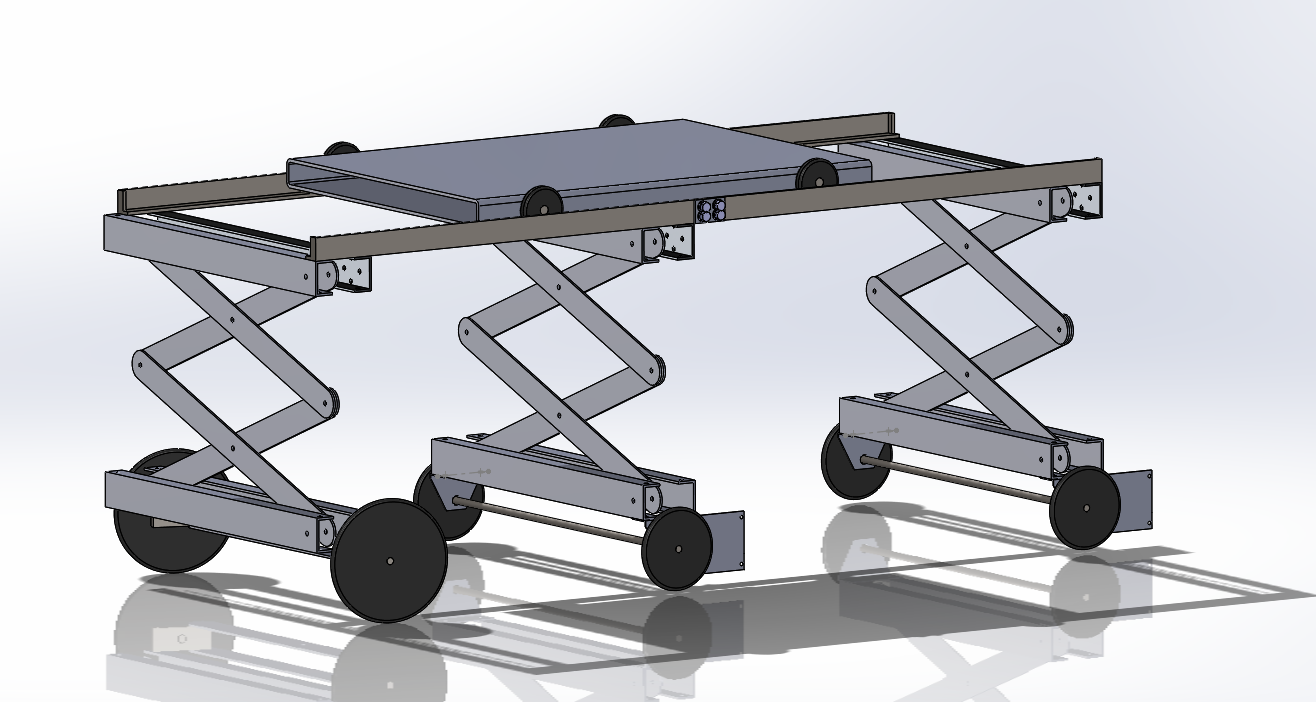
\includegraphics[width = 100mm]{04_gekozenconcept/eindconcept.png}
    \caption{3D-model Driepoter}
    \label{fig:driepoter_SW}
\end{figure}

In \cref{cha:bijlage_C} zijn de aanzichten van de driepoter afgebeeld met de bijbehorende hoofdmaten. 
